\chapter{Simulations of Cross-Beam Energy Transfer for Magnetised Direct-Drive}

This chapter describes a set of simulations which were conducted to understand the role of \ac{CBET} in magnetised, direct-drive implosions.
Magnetised \ac{ICF} is a promising route to achieving higher target gains, due to the reduction of thermal energy loss at stagnation and additional confinement of the alpha particles responsible for burn propagation.
For direct-drive implosions, magnetisation can significantly alter the coronal plasma profiles, due to the introduced anisotropy of thermal transport.
The \ac{IAW} dispersion relation, which mediates \ac{CBET} interactions, depends upon the background plasma and therefore significantly altered temperature and density profiles could alter the action of \ac{CBET}.
Before the development of \textsc{Solas}, no direct-drive suitable \ac{CBET} model existed, which was integrated into a \ac{Rad-MHD} code.
Therefore, the \textsc{Chimera}-\textsc{Solas} computational model has allowed the effect of magnetisation on \ac{CBET} to be studied for a direct-drive implosion.

The chapter begins with a review of experimental and computational work on magnetised \ac{ICF}, with a particular focus on magnetised direct-drive.
Work presented in this chapter focuses on the study of \textit{exploding-pusher} experiments.
These are very different implosions to the typical \textit{central hot-spot} ignition designs, presented in previous chapters, so a short summary of exploding pushers is also provided.
Simulation results are presented of 1-D and 2-D, unmagnetised exploding pushers, both with and without the effect of \ac{CBET}, which demonstrate that \ac{CBET} does significantly alter the implosion.
This is followed by an investigation of how various extended-\ac{MHD} terms affect the implosion, including the Nernst effect, the Lorentz force and resistive diffusion of the magnetic field.
Results are given of how magnetisation affects the \ac{CBET} interaction and ultimately how it changes the stagnation shape of the target.
The results presented, demonstrate that redistribution of deposited power due to \ac{CBET}, reduced the amplitude of the stagnation asymmetry, which originated from the polar beam configuration used, due to the presence of a field coil at the equator.
However, the reduction of asymmetry was consistent for different initial seed magnetic field values, and therefore \ac{CBET} was not observed to be sufficiently strongly affected by magnetisation, to lead to observable signatures in experimental measurements.
The chapter concludes with a summary of the work and suggestions of additional experimental configurations, which may leave a more significant signature of magnetisation altering \ac{CBET}.

\newpage

%###############################################################################################################################
%###############################################################################################################################
%###############################################################################################################################
\section{Magnetised Inertial Confinement Fusion and Exploding Pushers}%
\label{sec:Res2_MagICF}

This chapter begins with a review of published work that is relevant to the simulations which are presented.
Firstly, a short review of magnetised-\ac{ICF} is presented which reviews both the key concepts, existing studies and potential challenges of the design.
Both work on direct- and indirect drive is summarised, alongside recent theoretical progress on understanding how magnetisation can effect \ac{LPIs}.
The exploding pusher concept is then briefly explored to aid understanding of the implosion physics, which is markedly different to conventional hot-spot \ac{ICF}.

%################################################################################
%################################################################################
\subsection{Potential Benefits of Magnetisation}%
\label{sec:Res2_magbenefits}


\begin{figure}[t!]
    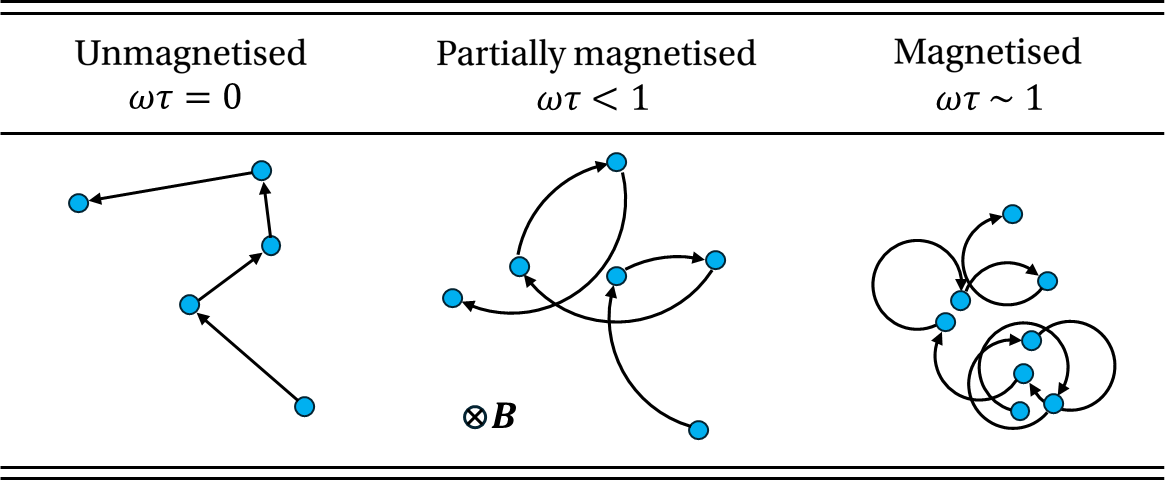
\includegraphics[width=0.75\linewidth]{Results2/Images/wt_collisions.png}
    \centering
    \caption{lol.}%
    \label{fig:Res2_Bose_magp2}
\end{figure}

\begin{figure}[t!]
    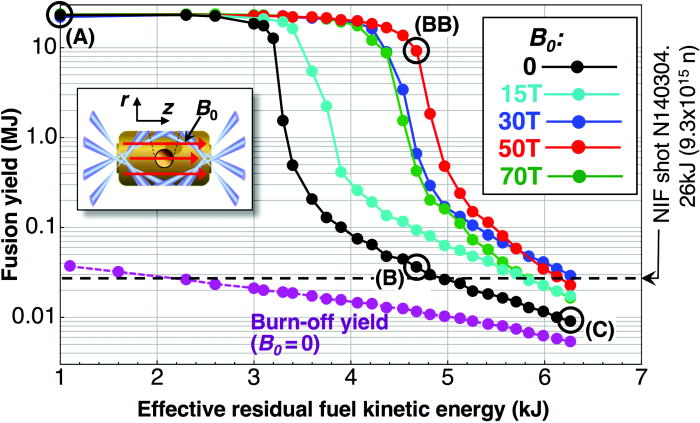
\includegraphics[width=0.75\linewidth]{Results2/Images/magicf_perkins.jpeg}
    \centering
    \caption{lol.
    Reused with permission from Ref.~\cite{perkins_potential_2017}.}%
    \label{fig:Res2_perkins_magicf}
\end{figure}


%################################################################################
%################################################################################
\subsection{Existing Studies of Magnetised-ICF}%
\label{sec:Res2_magicf_prevwork}


\begin{figure}[t!]
    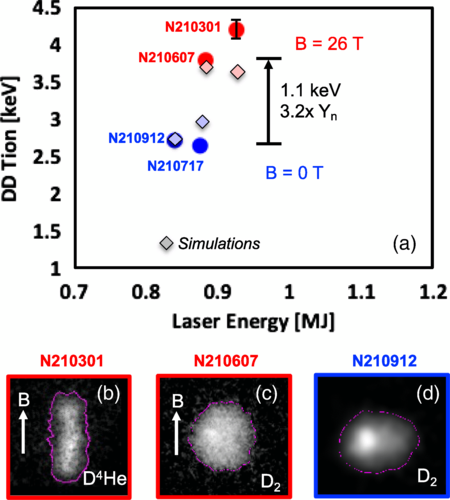
\includegraphics[width=0.5\linewidth]{Results2/Images/magnif_yield_inc.png}
    \centering
    \caption{lol.
    Reused with permission from Ref.~\cite{moody_increased_2022}.}%
    \label{fig:Res2_moody_magnif}
\end{figure}


\begin{figure}[t!]
    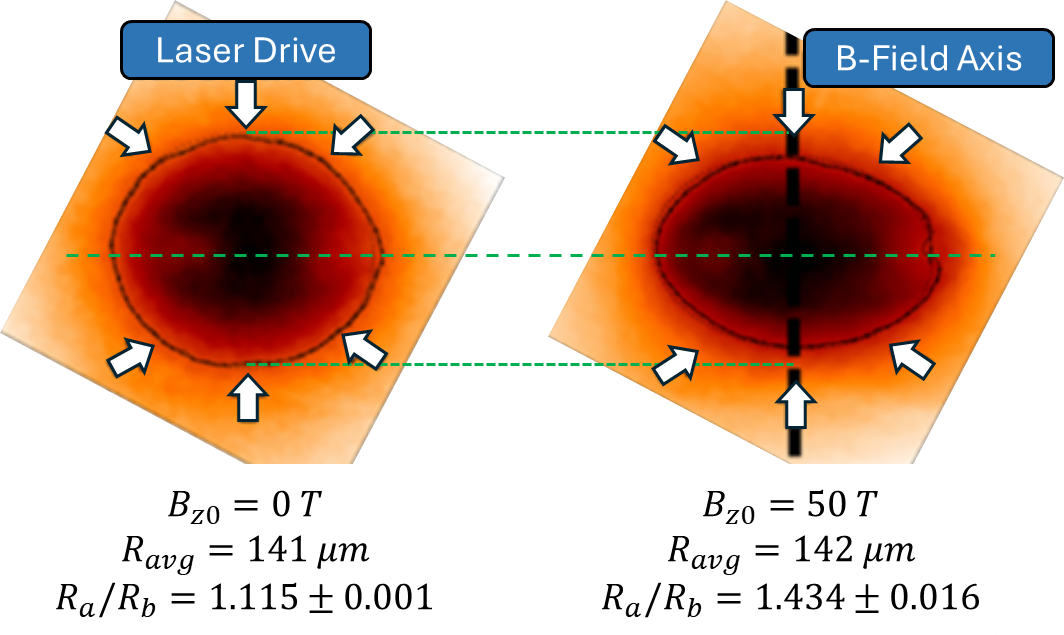
\includegraphics[width=0.6\linewidth]{Results2/Images/MagP2_Bose.png}
    \centering
    \caption{lol.
    Adapted with permission from Ref.~\cite{bose_effect_2022}.}%
    \label{fig:Res2_Bose_magp2}
\end{figure}


%################################################################################
%################################################################################
\subsection{Magnetised Laser-Plasma Instabilities}%
\label{sec:Res2_maglpis}



%################################################################################
%################################################################################
\subsection{The Exploding-Pusher Configuration}%
\label{sec:Res2_expl}



%################################################################################
%################################################################################
\subsection{Simulation Configuration}%
\label{sec:Res2_simconfig}


\begin{figure}[t!]
    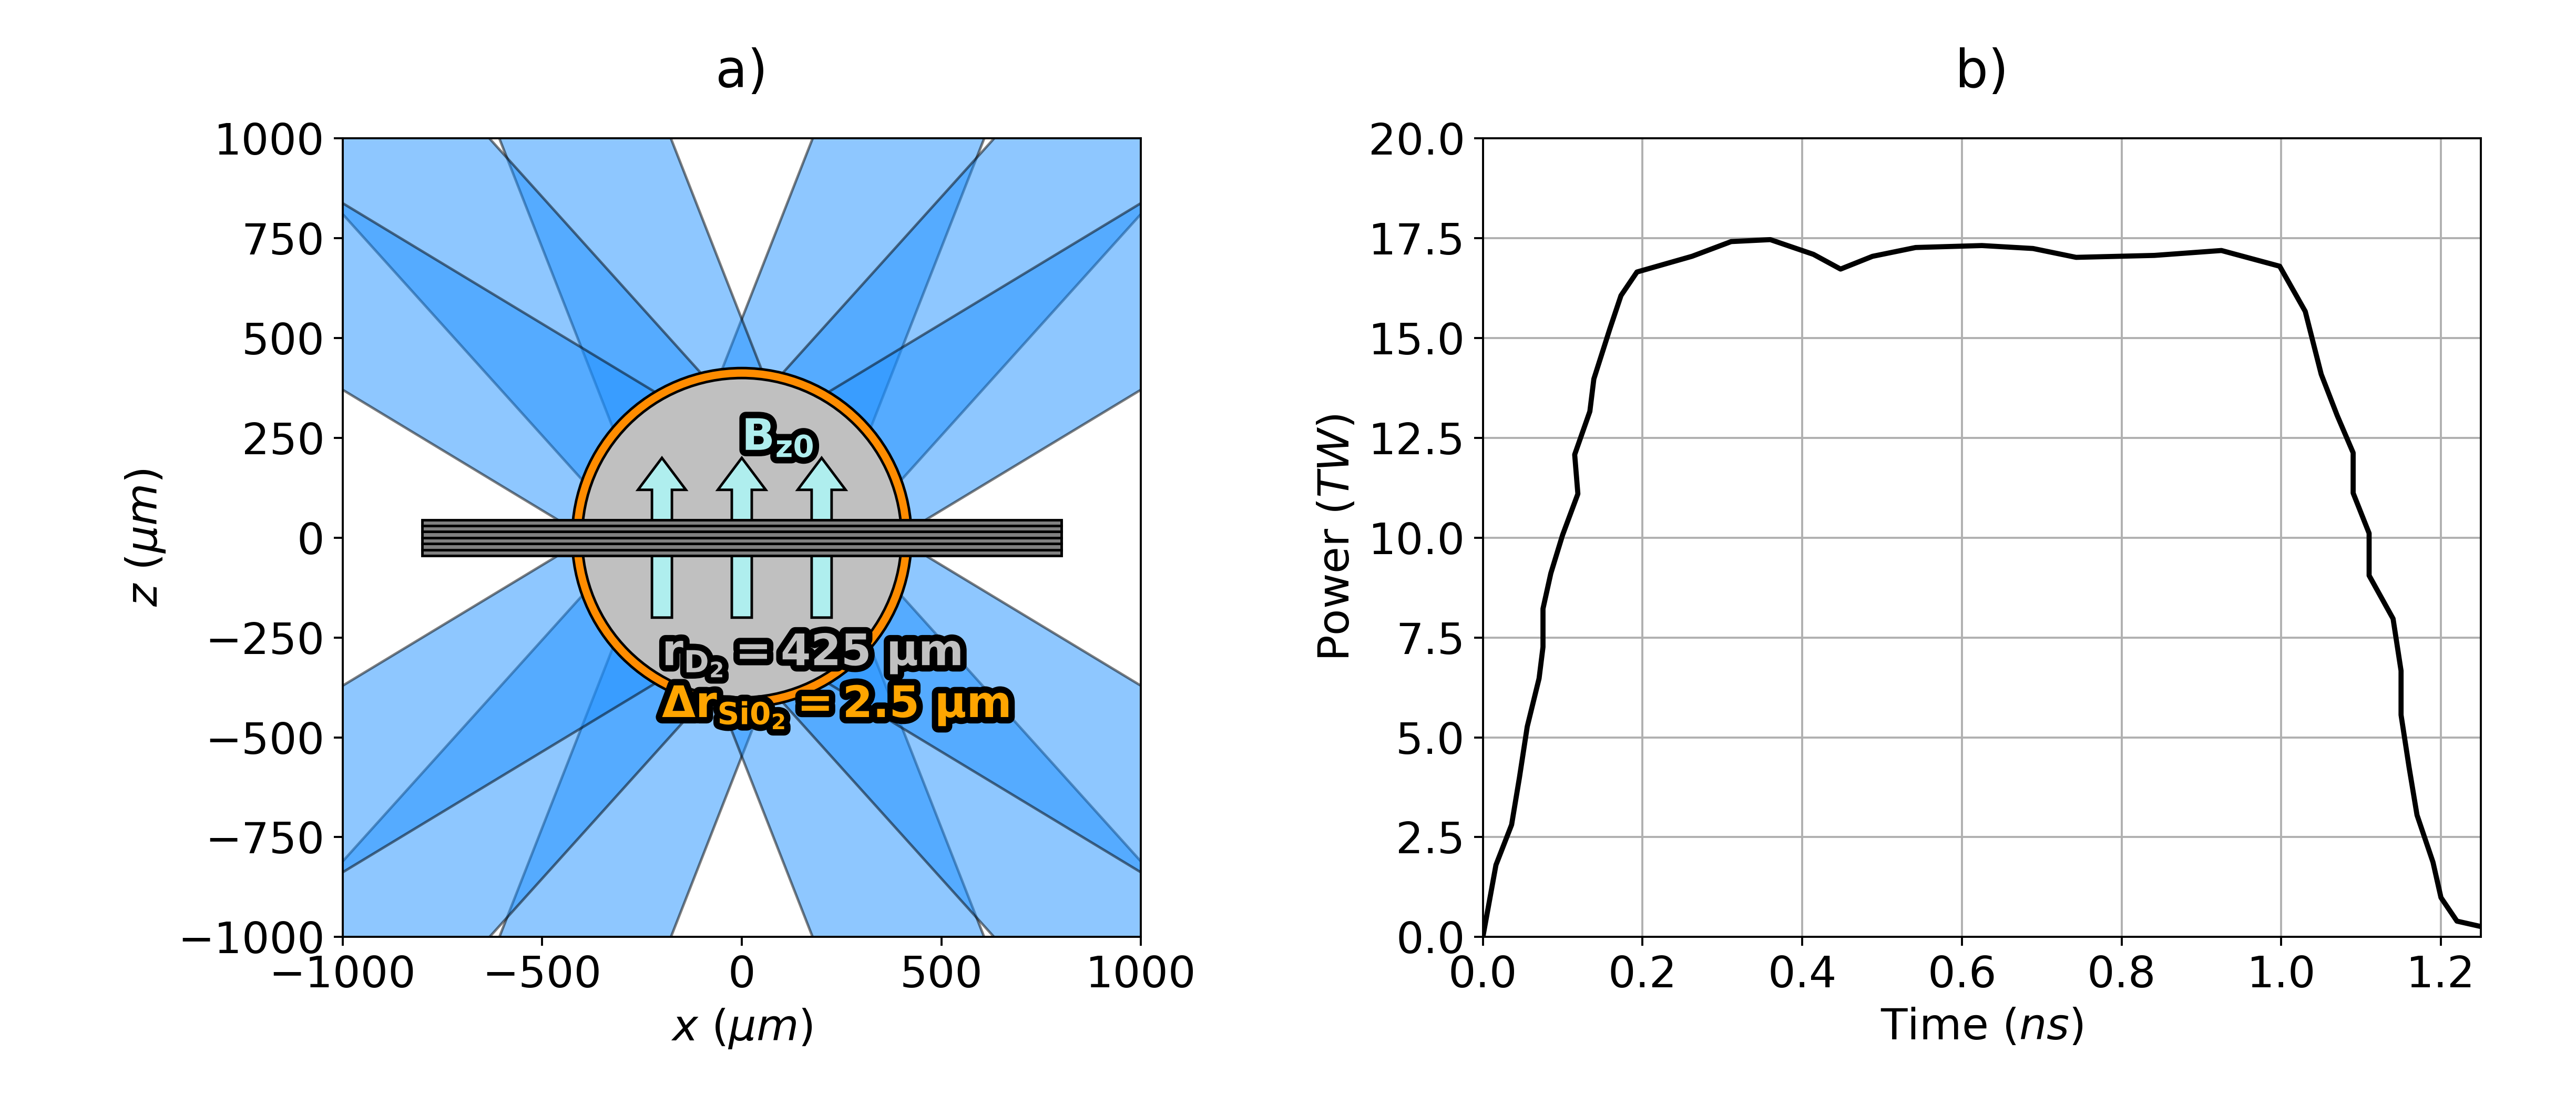
\includegraphics[width=\linewidth]{Results2/Images/magpdd_diagram_pulse.png}
    \centering
    \caption{lol.}%
    \label{fig:Res2_simconfig}
\end{figure}


%###############################################################################################################################
%###############################################################################################################################
%###############################################################################################################################
\section{Effect of Cross-Beam Energy Transfer in Unmagnetised Exploding Pushers}%
\label{sec:Res2_CBET_expl}

This section presents simulation results of the effect of \ac{CBET} in exploding pushers on \textsc{Omega}.
Both 1-D and 2-D \textsc{Chimera}-\textsc{Solas} simulations of 40-beam, polar driven exploding pusher experiments are presented, with a focus on how \ac{CBET} acts to change the implosion.
The 1-D results demonstrate that \ac{CBET} significantly reduces the coupled laser energy to the implosion from \dots to \dots.
Simulations conducted in 2-D, with a full 3-D raytrace and \ac{CBET} model, show that \ac{CBET} alters spatial profile of the laser deposition, reducing asymmetry in the drive.


%################################################################################
%################################################################################
\subsection{1-D Simulations}%
\label{sec:Res2_expl1D}



%################################################################################
%################################################################################
\subsection{2-D Simulations}%
\label{sec:Res2_expl2D}


\begin{figure}[t!]
    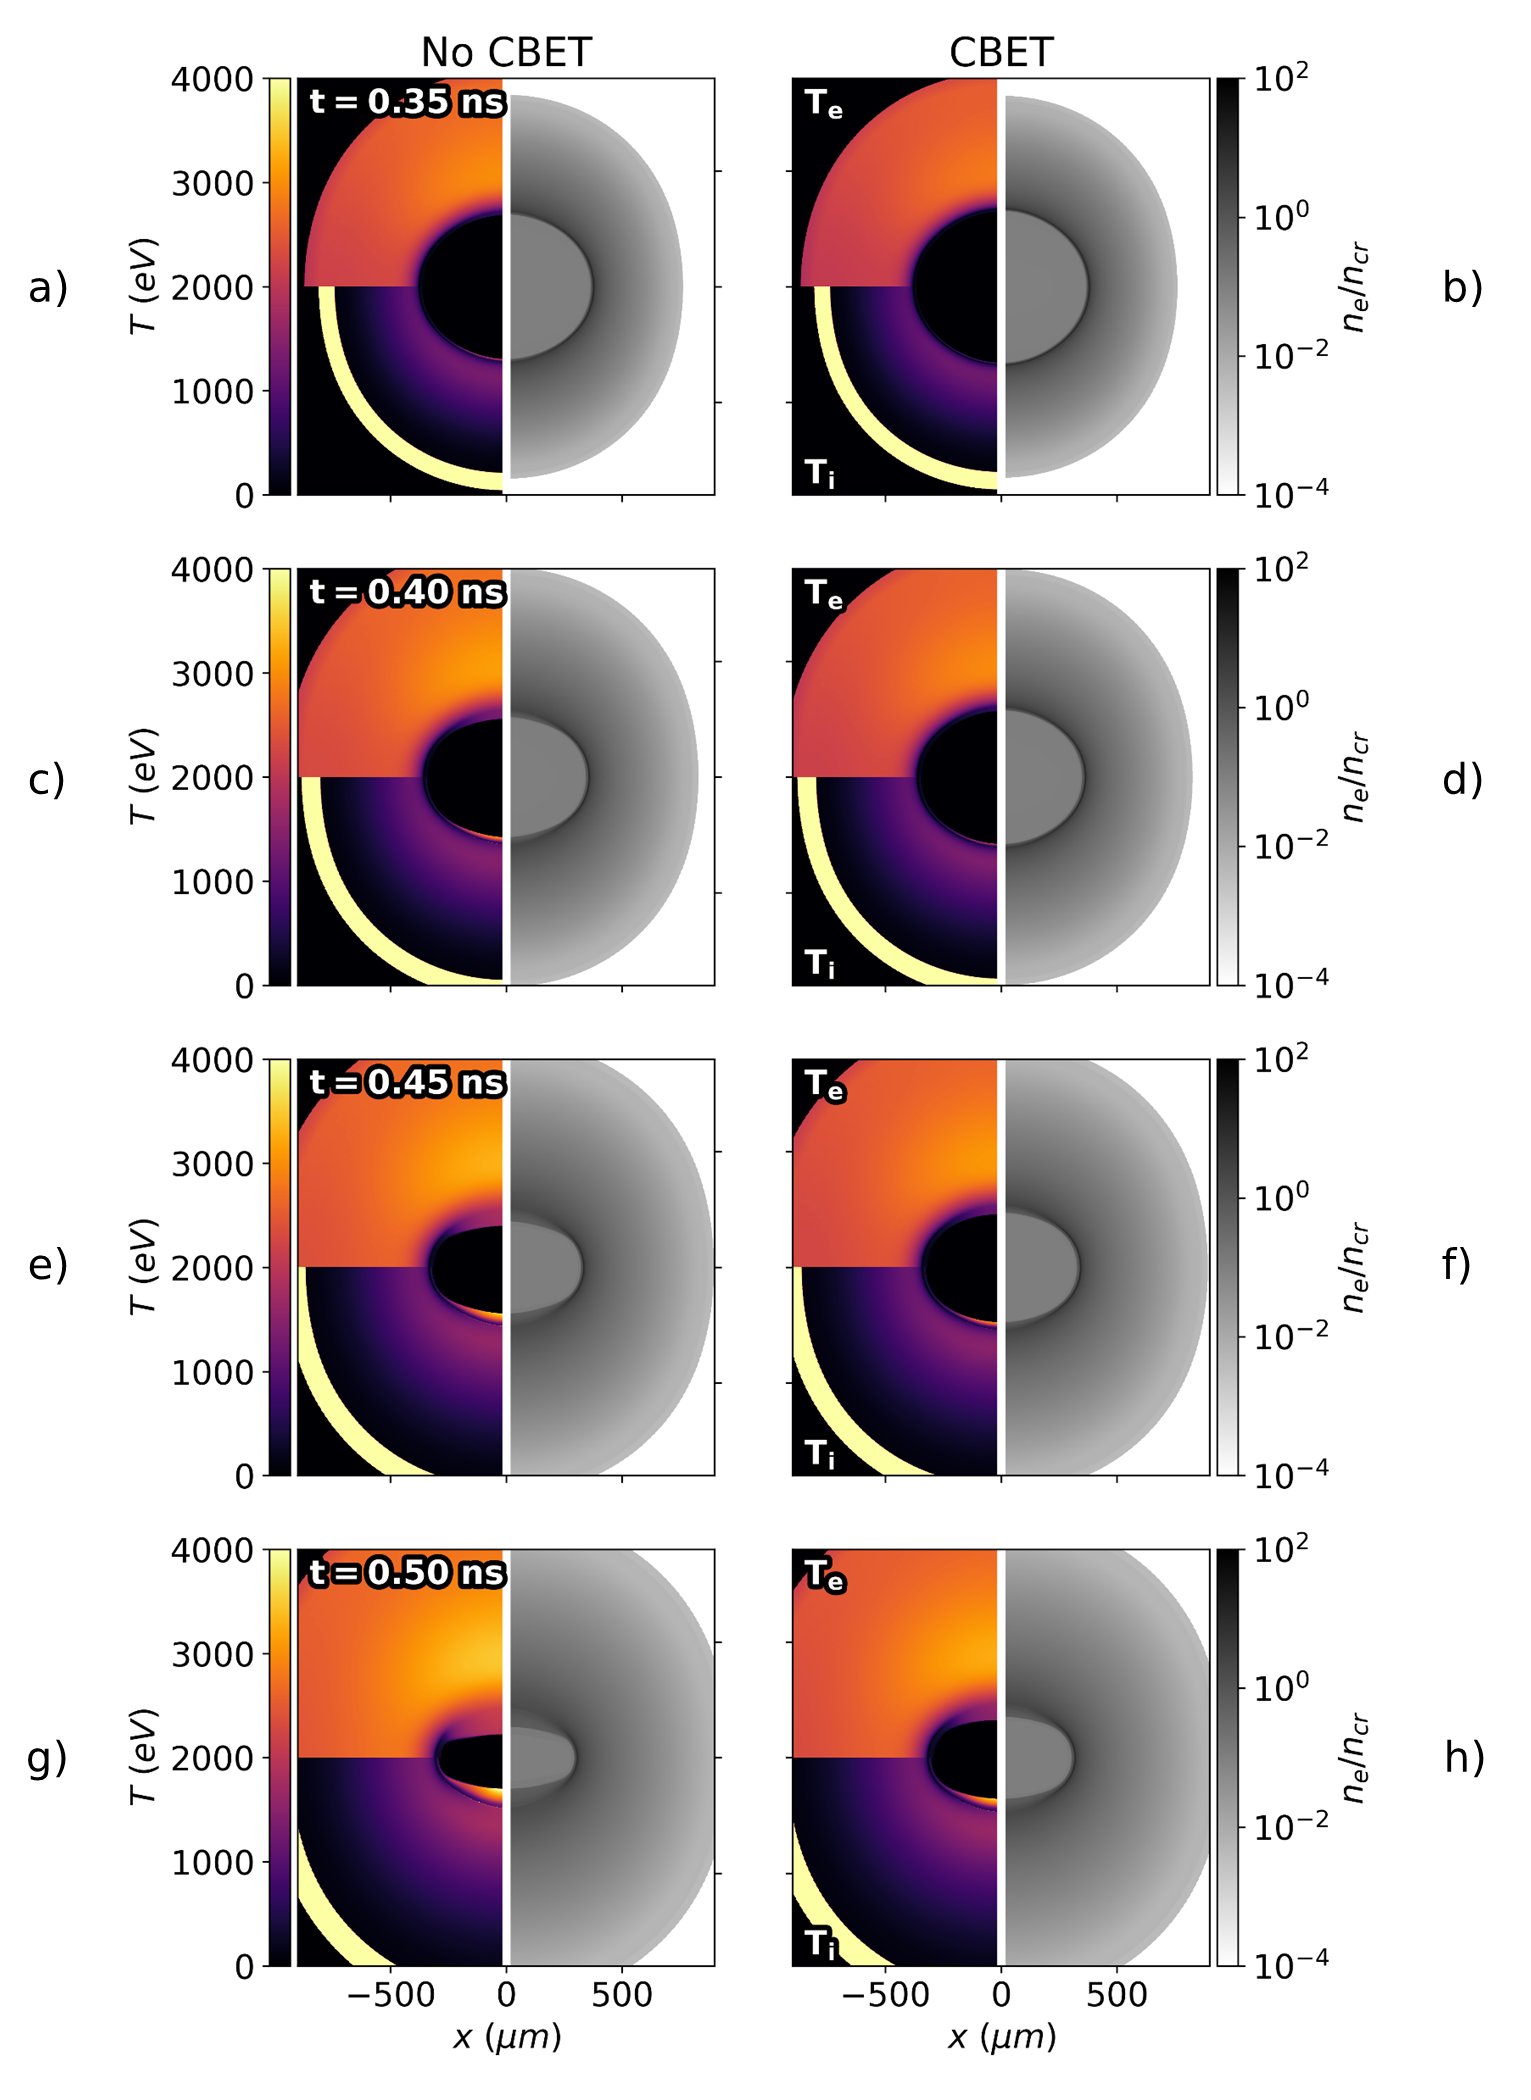
\includegraphics[width=0.9\linewidth]{Results2/Images/unmag_CBET_onoff.png}
    \centering
    \caption{lol.}%
    \label{fig:Res2_unmag_CBET_onoff}
\end{figure}



%###############################################################################################################################
%###############################################################################################################################
%###############################################################################################################################
\section{The Effect of Magnetisation on Exploding-Pusher Implosions}%
\label{sec:Res2_mag_unmag}

This section presents results of a study of the effect that extended-\ac{MHD} has on the 2-D exploding pusher simulations.
Simulations were conducted with varying initial magnetic field strengths and particular terms turned off and on to deduce what the important physical processes are.
Magnetised transport is important for both initial seed magnetic field implosions, resulting in large coronal Hall parameters and therefore significant anisotropy of the implosions.
The results demonstrate that (resistive diffusion and the Lorentz force have very little impact on the implosion physics, due to the bulk of the plasma being highly resistive and high-$\beta$ respectively)?????.
The Nernst advection of magnetic field ????????????????????


%################################################################################
%################################################################################
\subsection{In-Flight Field Structure}%
\label{sec:Res2_field_structure}


\begin{figure}[t!]
    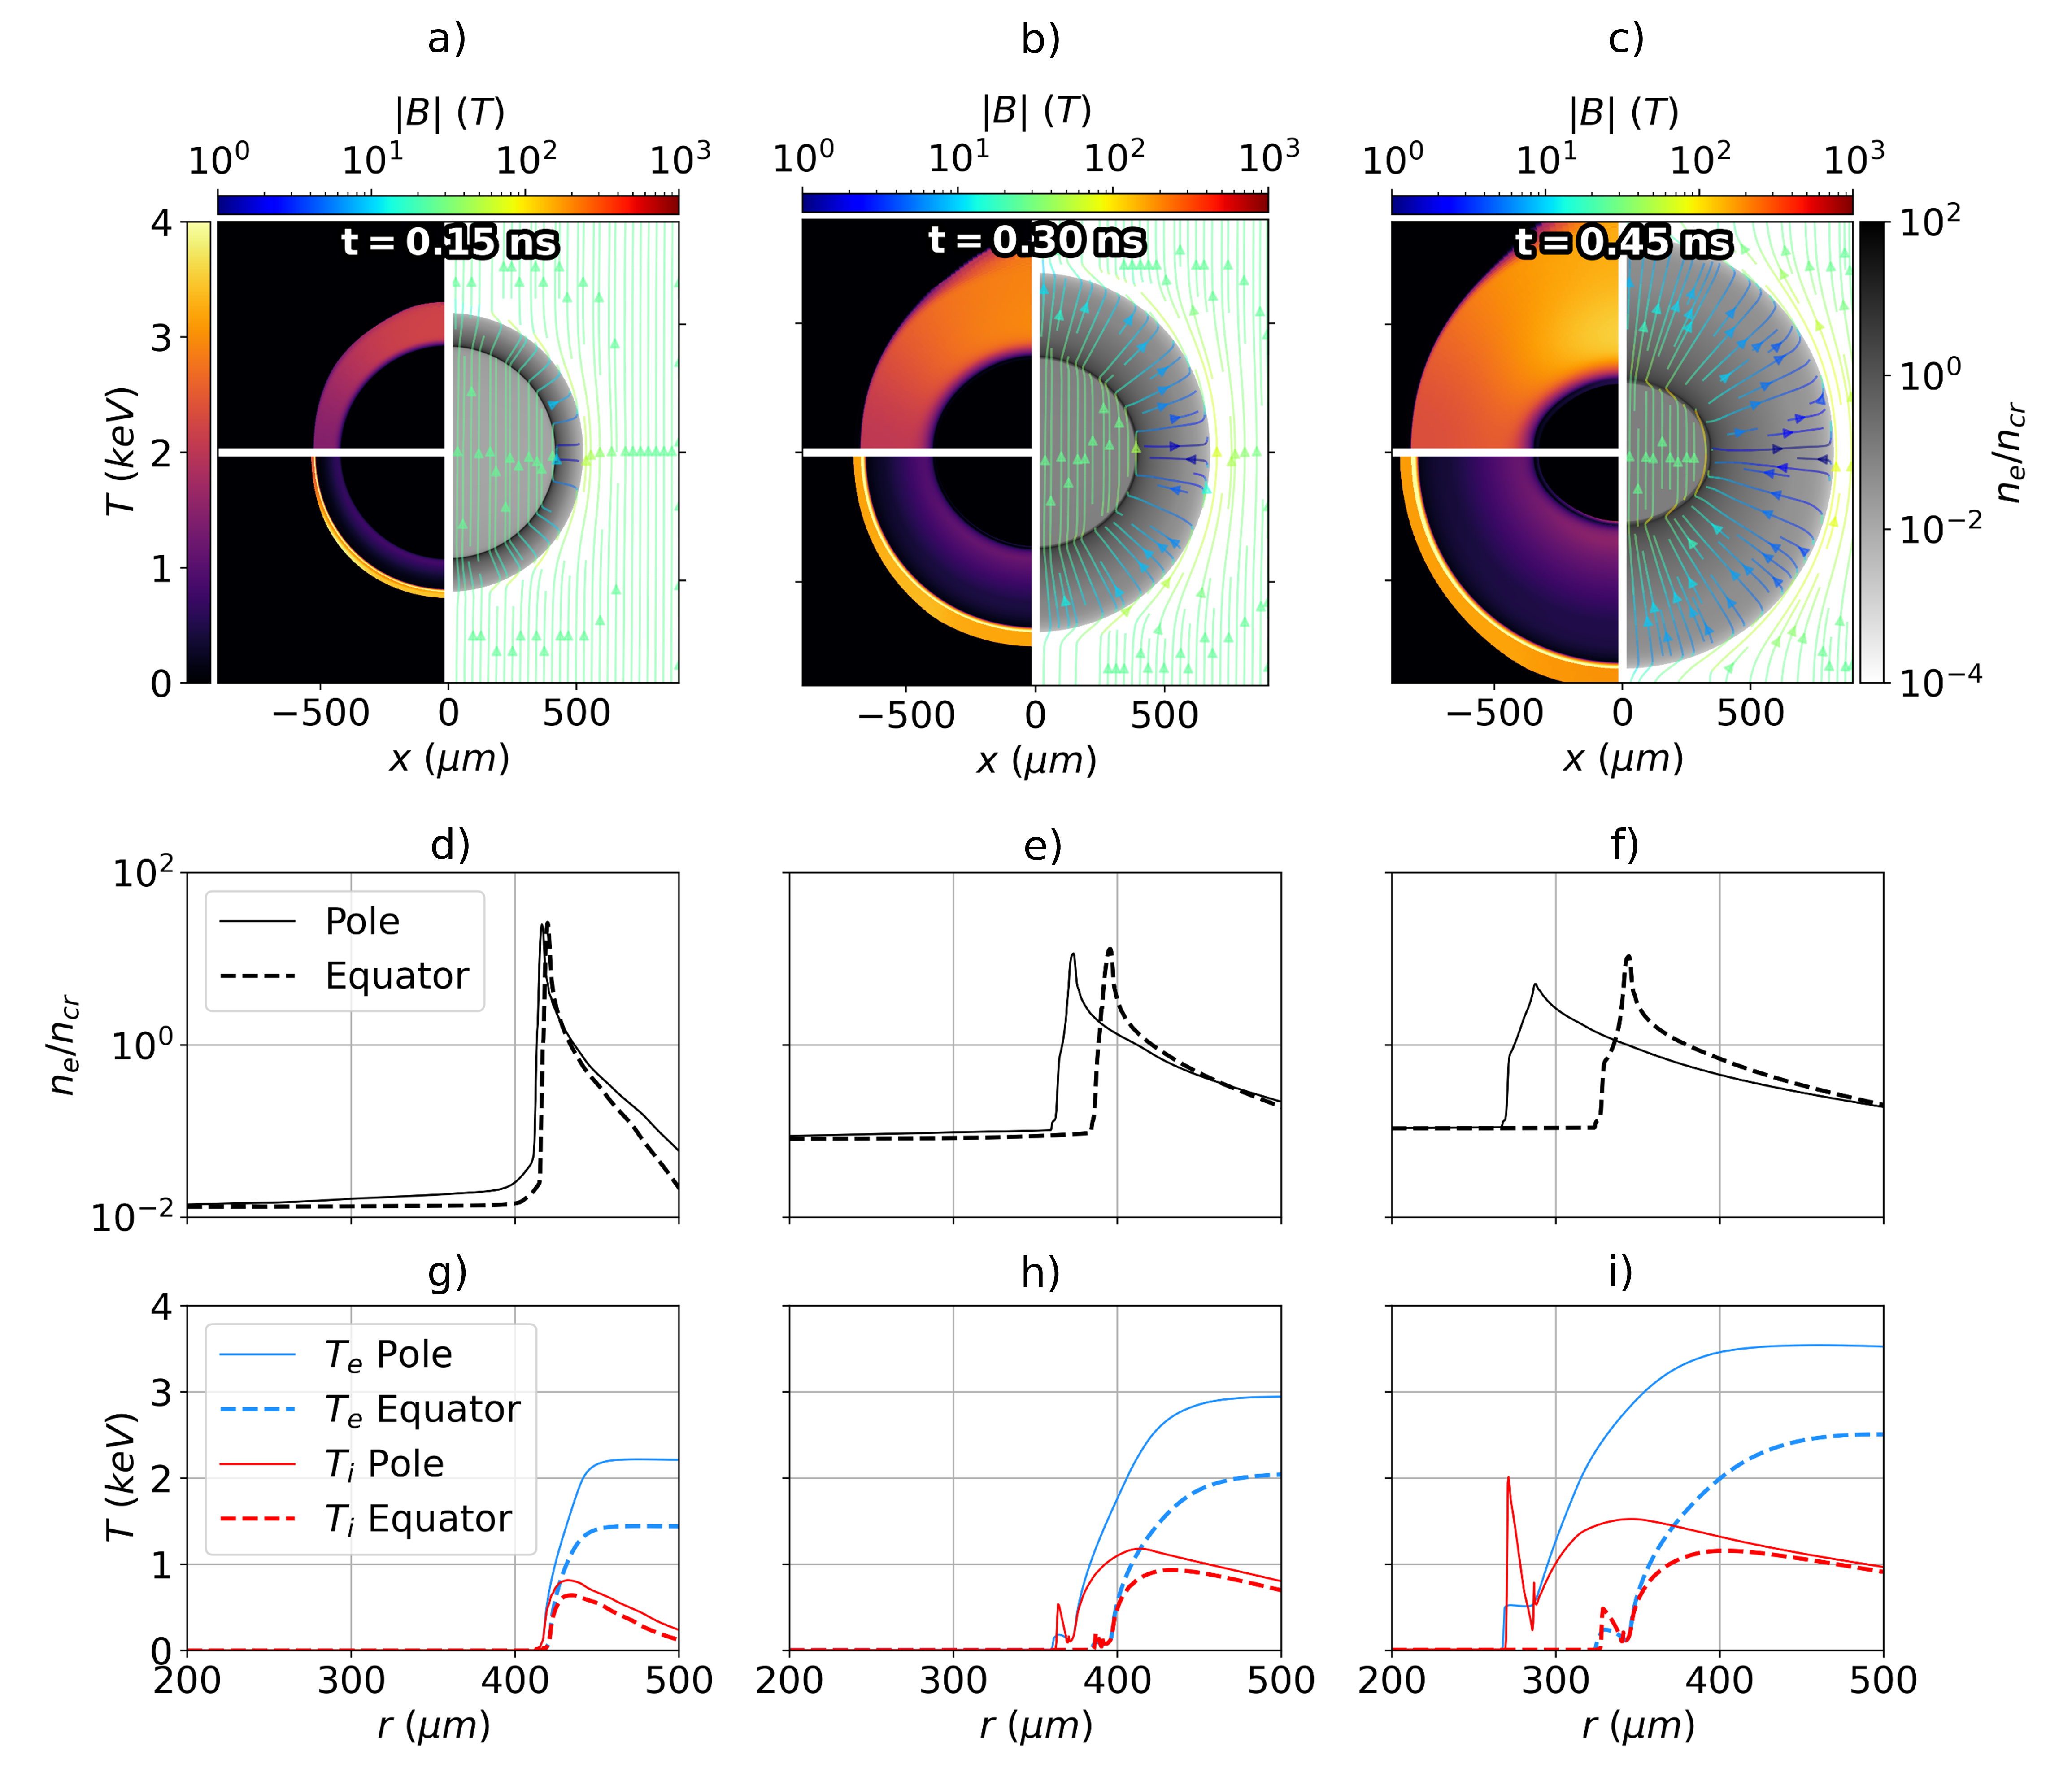
\includegraphics[width=\linewidth]{Results2/Images/mag_early_B_develop.png}
    \centering
    \caption{lol.}%
    \label{fig:Res2_mag_early_B_develop}
\end{figure}



%################################################################################
%################################################################################
\subsection{Anisotropic Thermal Conduction}%
\label{sec:Res2_aniso}



%################################################################################
%################################################################################
\subsection{The Nernst Effect}%
\label{sec:Res2_nernst}



%################################################################################
%################################################################################
\subsection{Resistive Diffusion and the Lorentz Force}%
\label{sec:Res2_resis}


\begin{figure}[t!]
    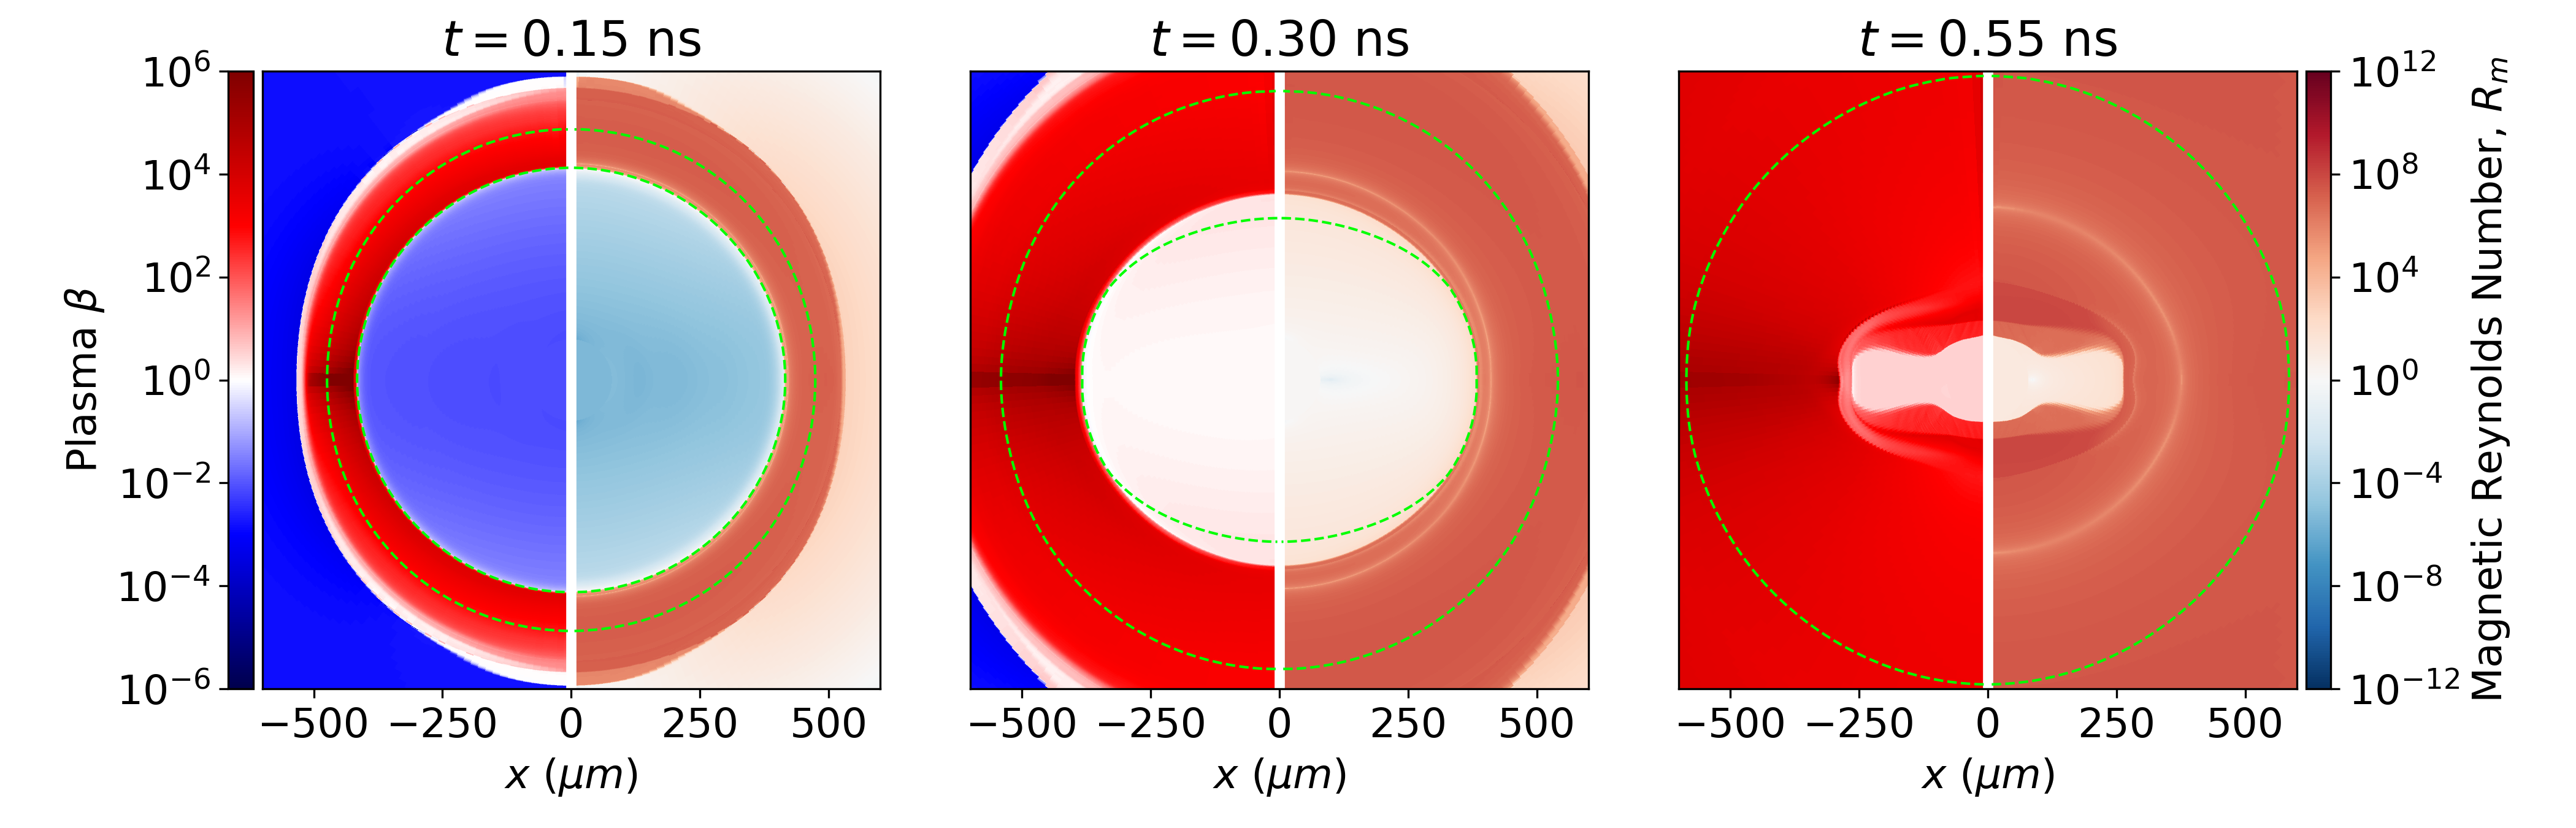
\includegraphics[width=\linewidth]{Results2/Images/magmag_beta_Rm.png}
    \centering
    \caption{lol.}%
    \label{fig:Res2_magmag_beta_Rm}
\end{figure}



%###############################################################################################################################
%###############################################################################################################################
%###############################################################################################################################
\section{The Effect of Magnetisation on Cross-Beam Energy Transfer and Stagnation}%
\label{sec:Res2_mag_on_CBET}


\begin{figure}[t!]
    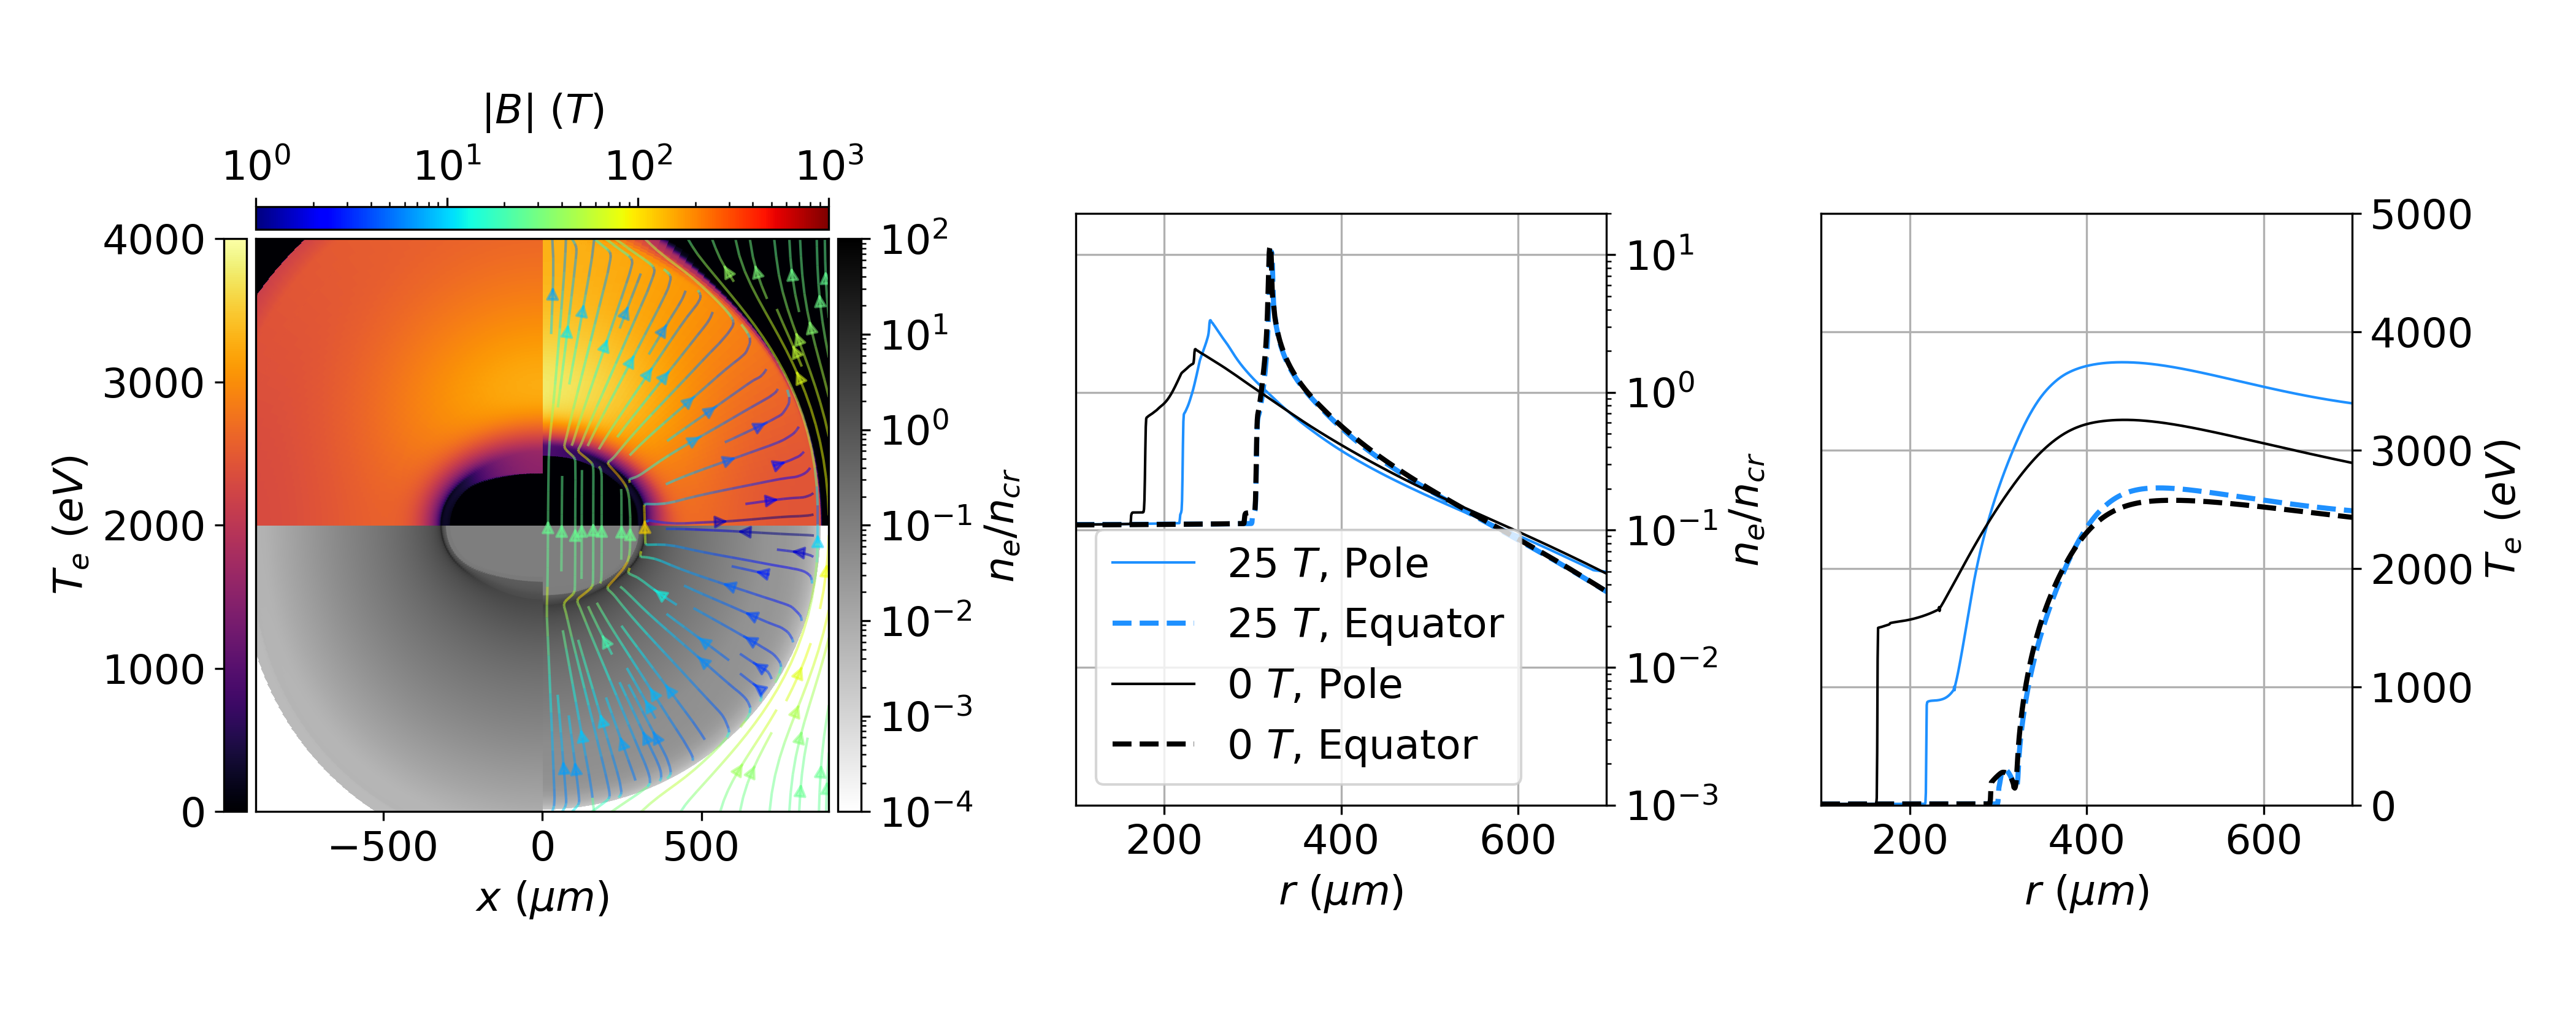
\includegraphics[width=\linewidth]{Results2/Images/ne_te_Bstream_comp_alt050.png}
    \centering
    \caption{lol.}%
    \label{fig:Res2_ne_te_Bstream_comp_alt050}
\end{figure}

This section presents results on how the magnetisation of the corona affects both \ac{CBET} scattering and the stagnation shape of the implosion.
As was shown in the previous sections, the laser geometry leads to a significant mode $\ell=2$ in the coronal plasma conditions, which is significantly amplified by anisotropic thermal conduction when magnetised.
This long-wavelength perturbation is slightly reduced by \ac{CBET}, consistent with existing literature on how \ac{CBET} mitigates $\ell=1$ asymmetries~\cite{colaitis_inverse_2021}.
`No-\ac{CBET}' simulations were conducted, for which the coupled energy was kept the same as the equivalent \ac{CBET} simulation, \textit{i.e.} so \ac{CBET} only acted to redistribute the deposited power, rather than reduce its magnitude.
These results showed that the increasingly anisotropic coronal plasma profiles for increasing seed magnetic field strengths did lead to changes in the \ac{CBET} scattering, this was too small an effect to lead to experimentally observable changes in behaviour.

%################################################################################
%################################################################################
\subsection{Analysis and Key Definitions}%
\label{sec:Res2_analysis_definitions}

\begin{figure}[t!]
    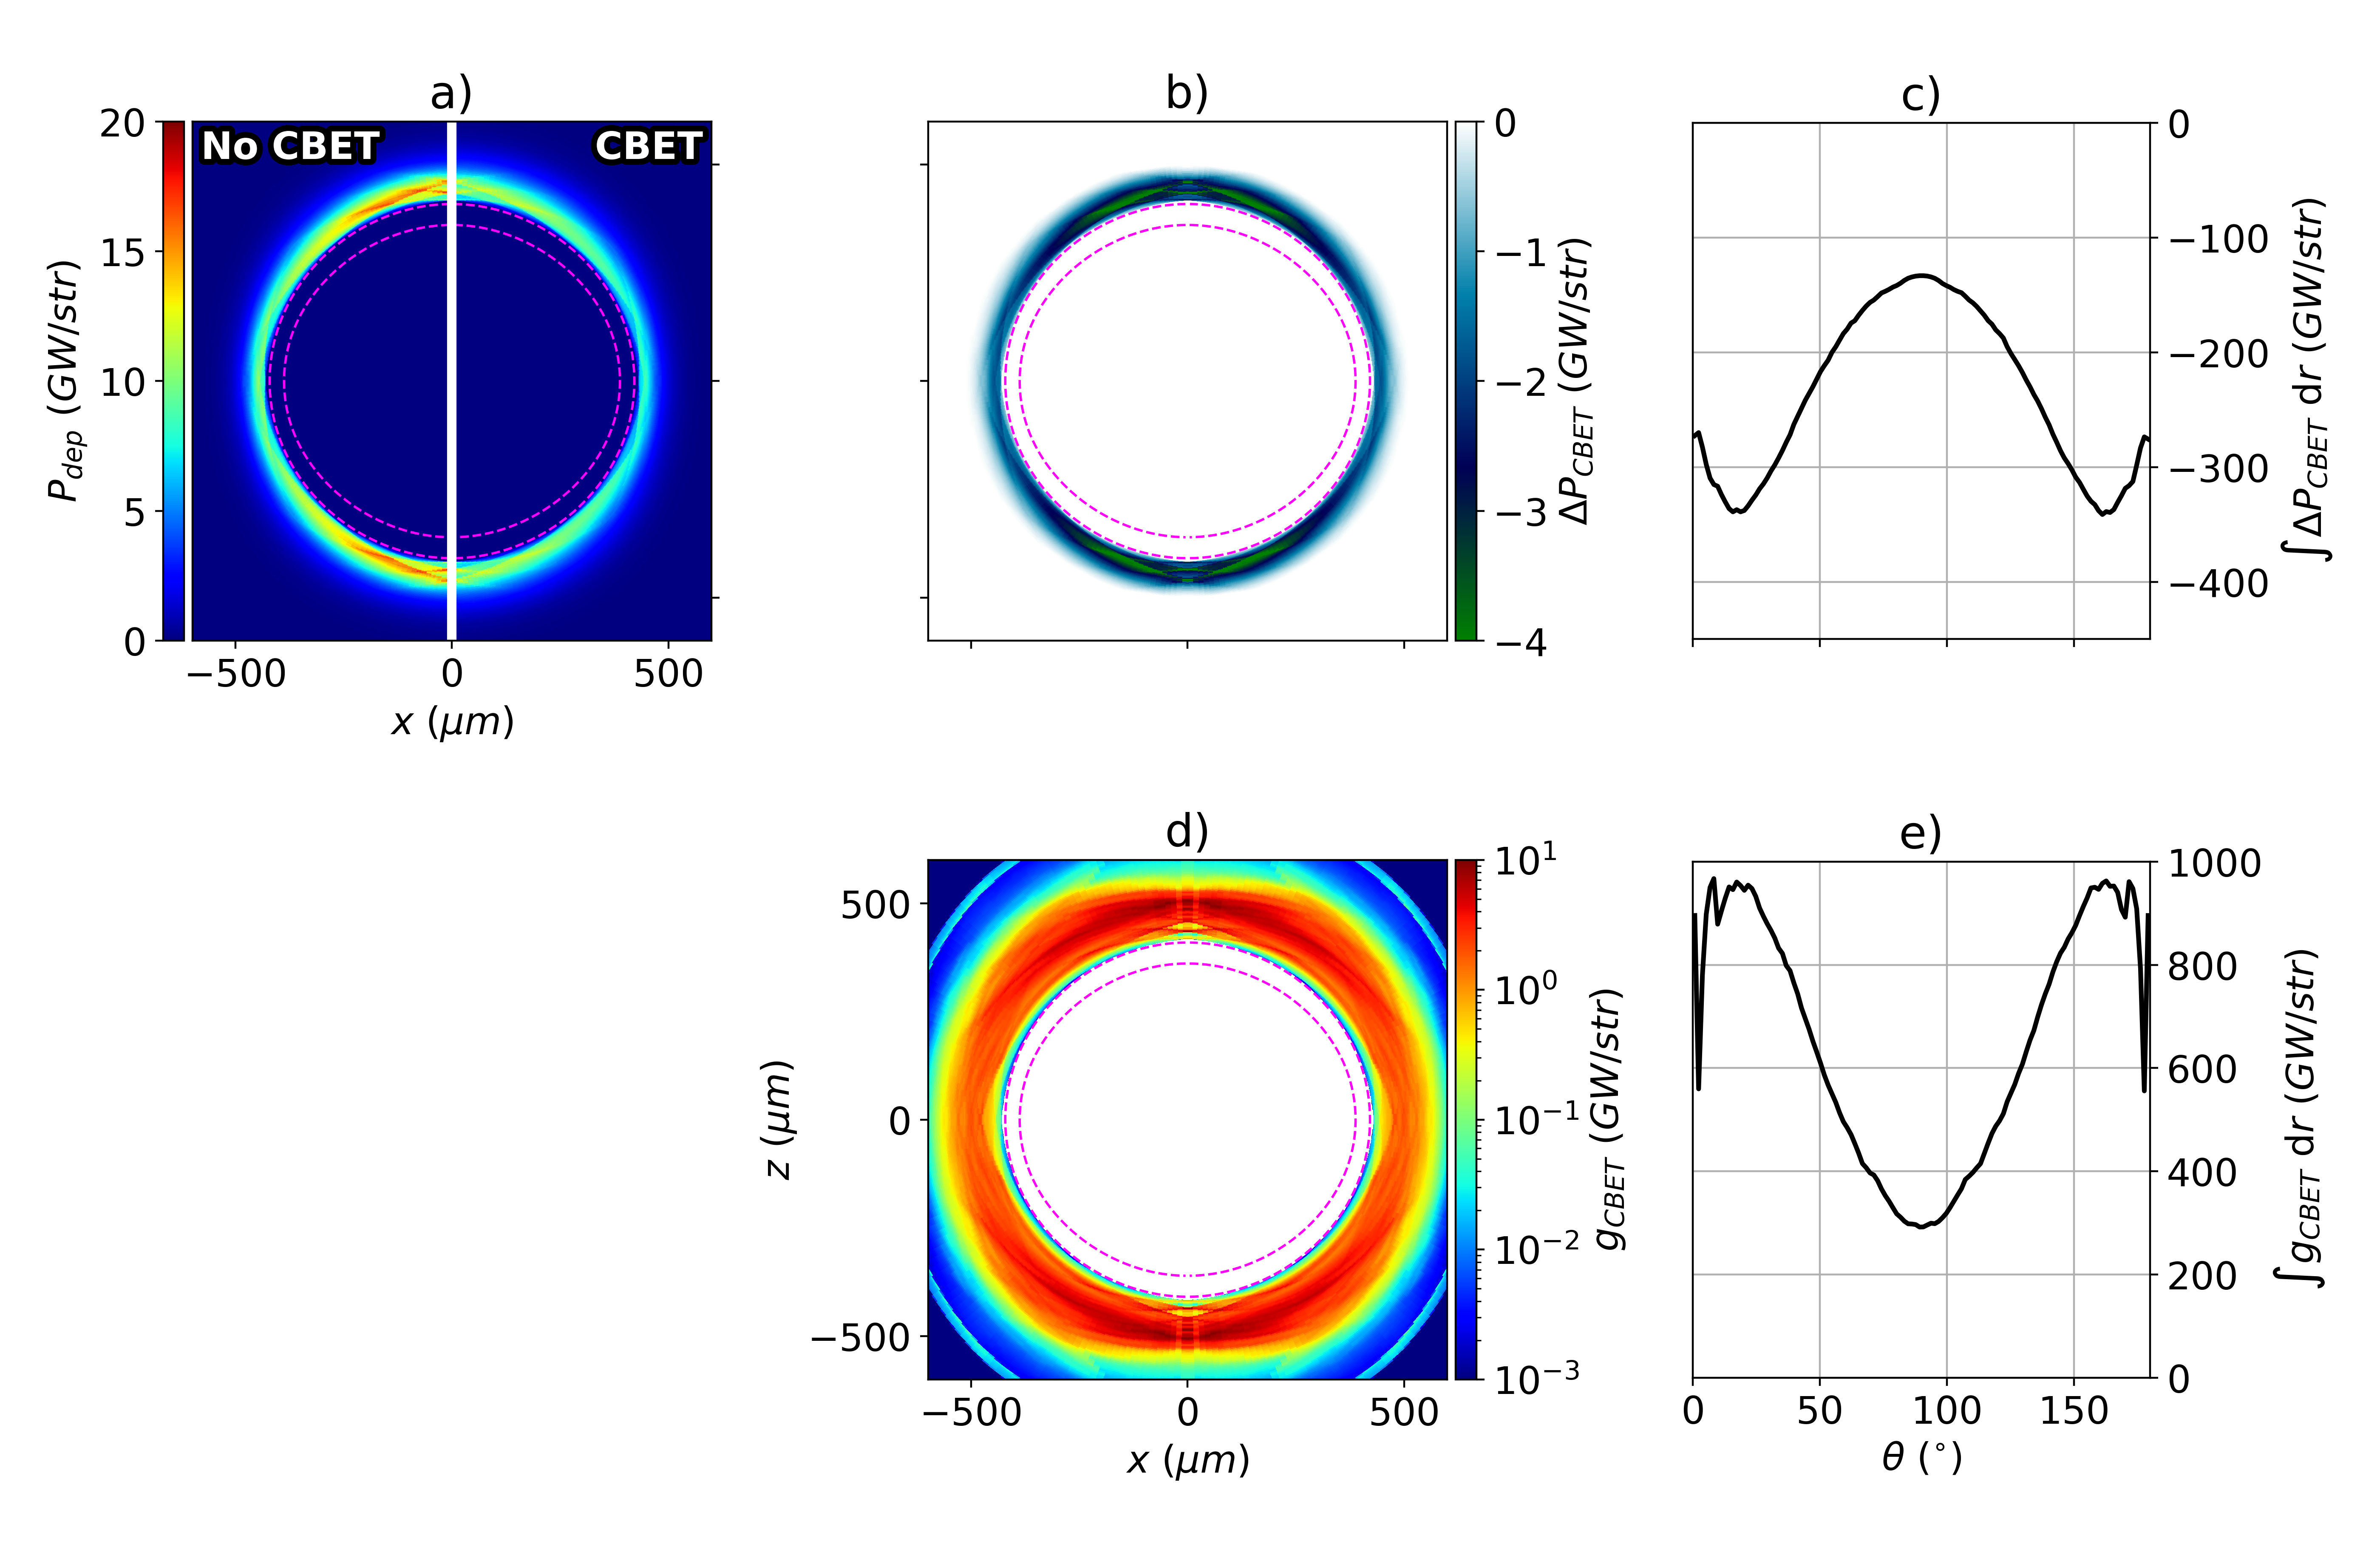
\includegraphics[width=\linewidth]{Results2/Images/magcbet_analysis.png}
    \centering
    \caption{lol.}%
    \label{fig:Res2_magcbet_analysis}
\end{figure}


%################################################################################
%################################################################################
\subsection{Spatial Change of CBET and Deposition from Magnetisation}%
\label{sec:Res2_mag_on_cbet_change}

\bgroup%
\def\arraystretch{1.3}%  1 is the default, change whatever you need
% Please add the following required packages to your document preamble:
% \usepackage{multirow}
\begin{table}[]
    \centering
    \caption{Results of all Simulations. In the CBET column, `$\sim$' indicates CBET affecting the magnitude, but \textit{not} spatial location, of deposition.}
    \begin{tabular}{cccccccccc}
        \hhline{==========}
        Run & Dim. & CBET   & Note      & \begin{tabular}[c]{@{}c@{}}$B_{z0}$\\ $(\mathrm{T})$\end{tabular} & \begin{tabular}[c]{@{}c@{}}$t_b$\\ $(\mathrm{ns})$\end{tabular} & \begin{tabular}[c]{@{}c@{}}$\langle T_i \rangle$\\ (keV)\end{tabular} & \begin{tabular}[c]{@{}c@{}}$Y_n$\\ $(\times10^{10}$\end{tabular} & \begin{tabular}[c]{@{}c@{}}$\Delta_b$\\ (ps)\end{tabular} & $R_2/R_1$              \\ \hline
        1   & 1-D  & Off    & -         & 0                                                                 & 0.69                                                            & 14.66                                                                 & 11.62                                                            & 87                                                        & $1.00_{-0.00}^{+0.00}$ \\
        2   & 1-D  & On     & -         & 0                                                                 &                                                                 &                                                                       &                                                                  &                                                           & $1.00_{-0.00}^{+0.00}$ \\
        3   & 2-D  & Off    & -         & 0                                                                 & 0.71                                                            & 8.44                                                                  & 6.20                                                             & 148                                                       & $2.96_{-0.19}^{+0.20}$ \\
        4   & 2-D  & $\sim$ & -         & 0                                                                 & 0.75                                                            & 7.61                                                                  & 5.23                                                             & 153                                                       & $3.26_{-0.23}^{+0.25}$ \\
        5   & 2-D  & On     & -         & 0                                                                 & 0.75                                                            & 7.77                                                                  & 5.46                                                             & 148                                                       & $3.23_{-0.23}^{+0.25}$ \\
        6   & 2-D  & Off    & -         & 25                                                                & 0.74                                                            & 7.26                                                                  & 4.73                                                             & 130                                                       & $3.80_{-0.33}^{+0.41}$ \\
        7   & 2-D  & $\sim$ & -         & 25                                                                & 0.78                                                            & 6.58                                                                  & 4.14                                                             & 125                                                       & $4.55_{-0.43}^{+0.50}$ \\
        8   & 2-D  & On     & -         & 25                                                                & 0.78                                                            & 6.72                                                                  & 4.44                                                             & 123                                                       & $4.32_{-0.41}^{+0.47}$ \\
        9   & 2-D  & Off    & -         & 50                                                                & 0.73                                                            & 6.82                                                                  & 3.73                                                             & 134                                                       & $4.40_{-0.38}^{0.43}$  \\
        10  & 2-D  & $\sim$ & -         & 50                                                                & 0.78                                                            & 6.30                                                                  & 3.30                                                             & 130                                                       & $4.92_{-0.48}^{0.56}$  \\
        11  & 2-D  & On     & -         & 50                                                                & 0.78                                                            & 6.37                                                                  & 3.52                                                             & 129                                                       & $4.79_{-0.47}^{+0.55}$ \\
        12  & 2-D  & Off    & No Aniso. & 25                                                                & 0.81                                                            & 6.40                                                                  & 5.02                                                             & 118                                                       & $3.14_{-0.50}^{+0.68}$ \\
        13  & 2-D  & Off    & No Lor.   & 25                                                                & 0.74                                                            & 7.29                                                                  & 4.77                                                             & 131                                                       & $3.80_{-0.33}^{+0.41}$ \\
        14  & 2-D  & Off    & No Nern.  & 25                                                                & 0.73                                                            & 7.41                                                                  & 4.85                                                             & 130                                                       & $3.74_{-0.32}^{+0.38}$ \\
        15  & 2-D  & Off    & No Resis. & 25                                                                & 0.73                                                            & 7.07                                                                  & 4.59                                                             & 132                                                       & $3.84_{-0.33}^{+0.42}$ \\ \hhline{==========}
\end{tabular}
\end{table}
\egroup%

%################################################################################
%################################################################################
\subsection{Stagnation Profiles}%
\label{sec:Res2_stgnation_profiles}


\begin{figure}[t!]
    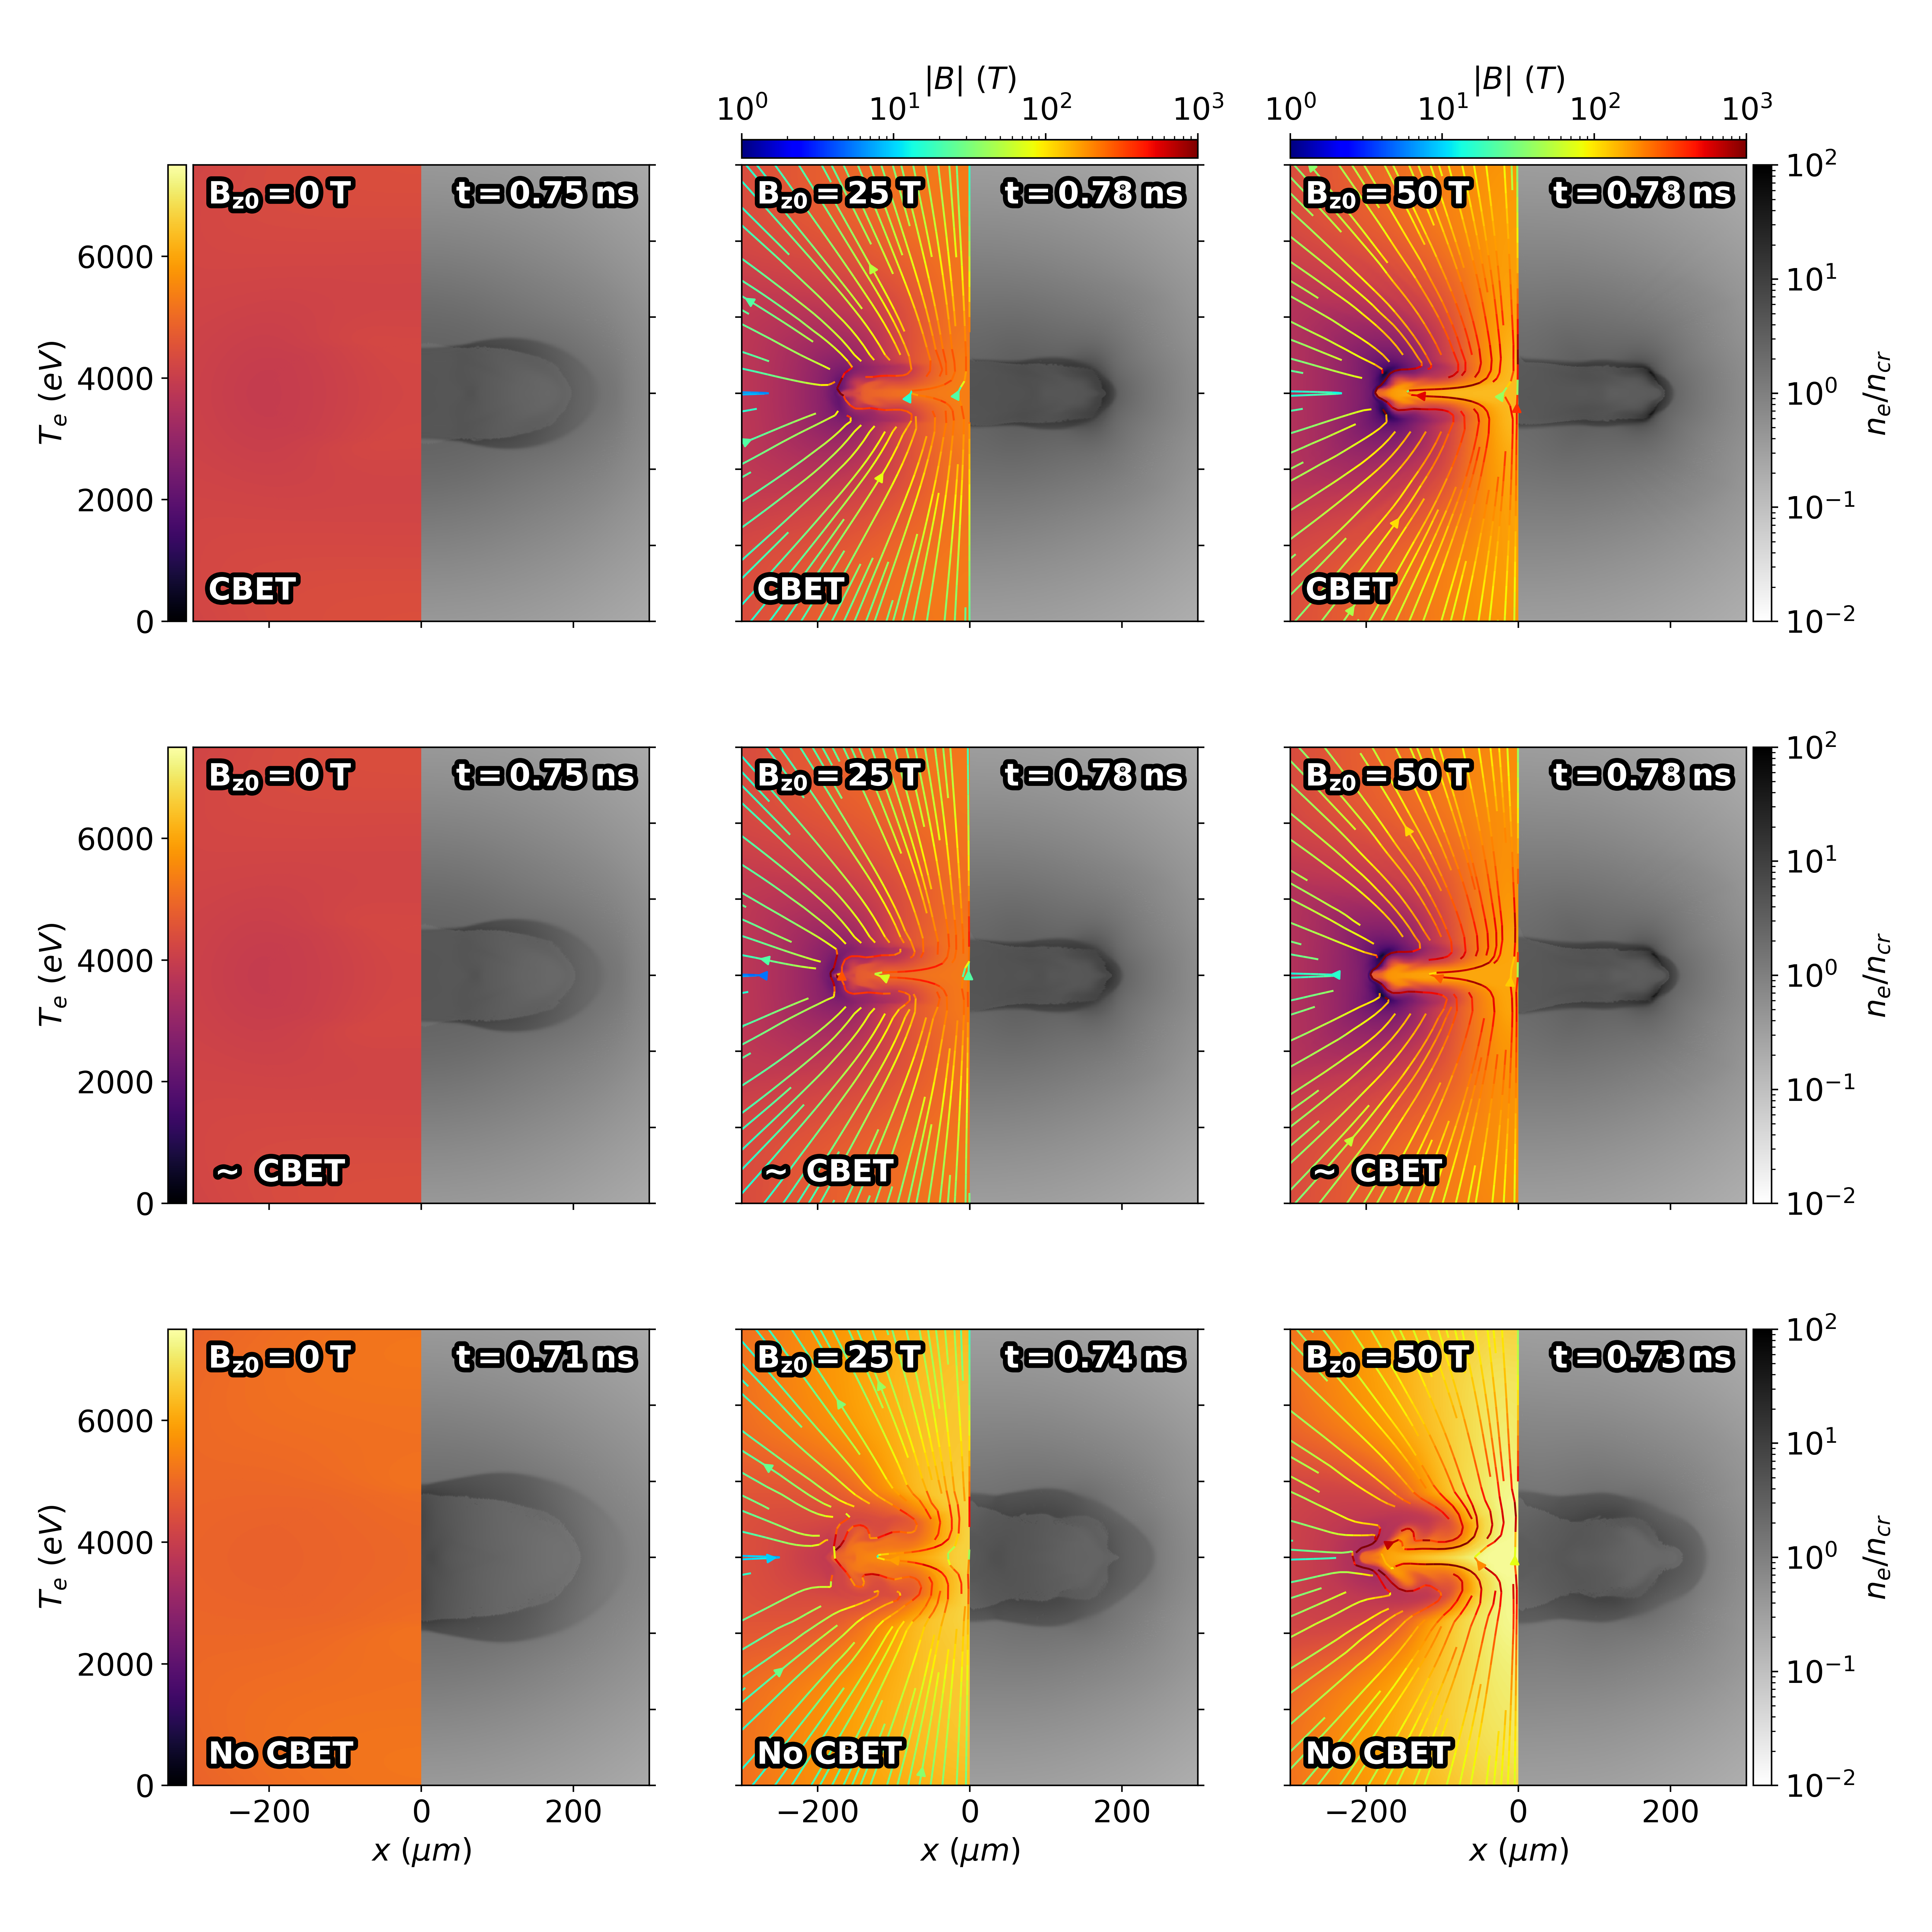
\includegraphics[width=\linewidth]{Results2/Images/allall_stagnation.png}
    \centering
    \caption{lol.}%
    \label{fig:Res2_allall_stagnation}
\end{figure}


\begin{figure}[t!]
    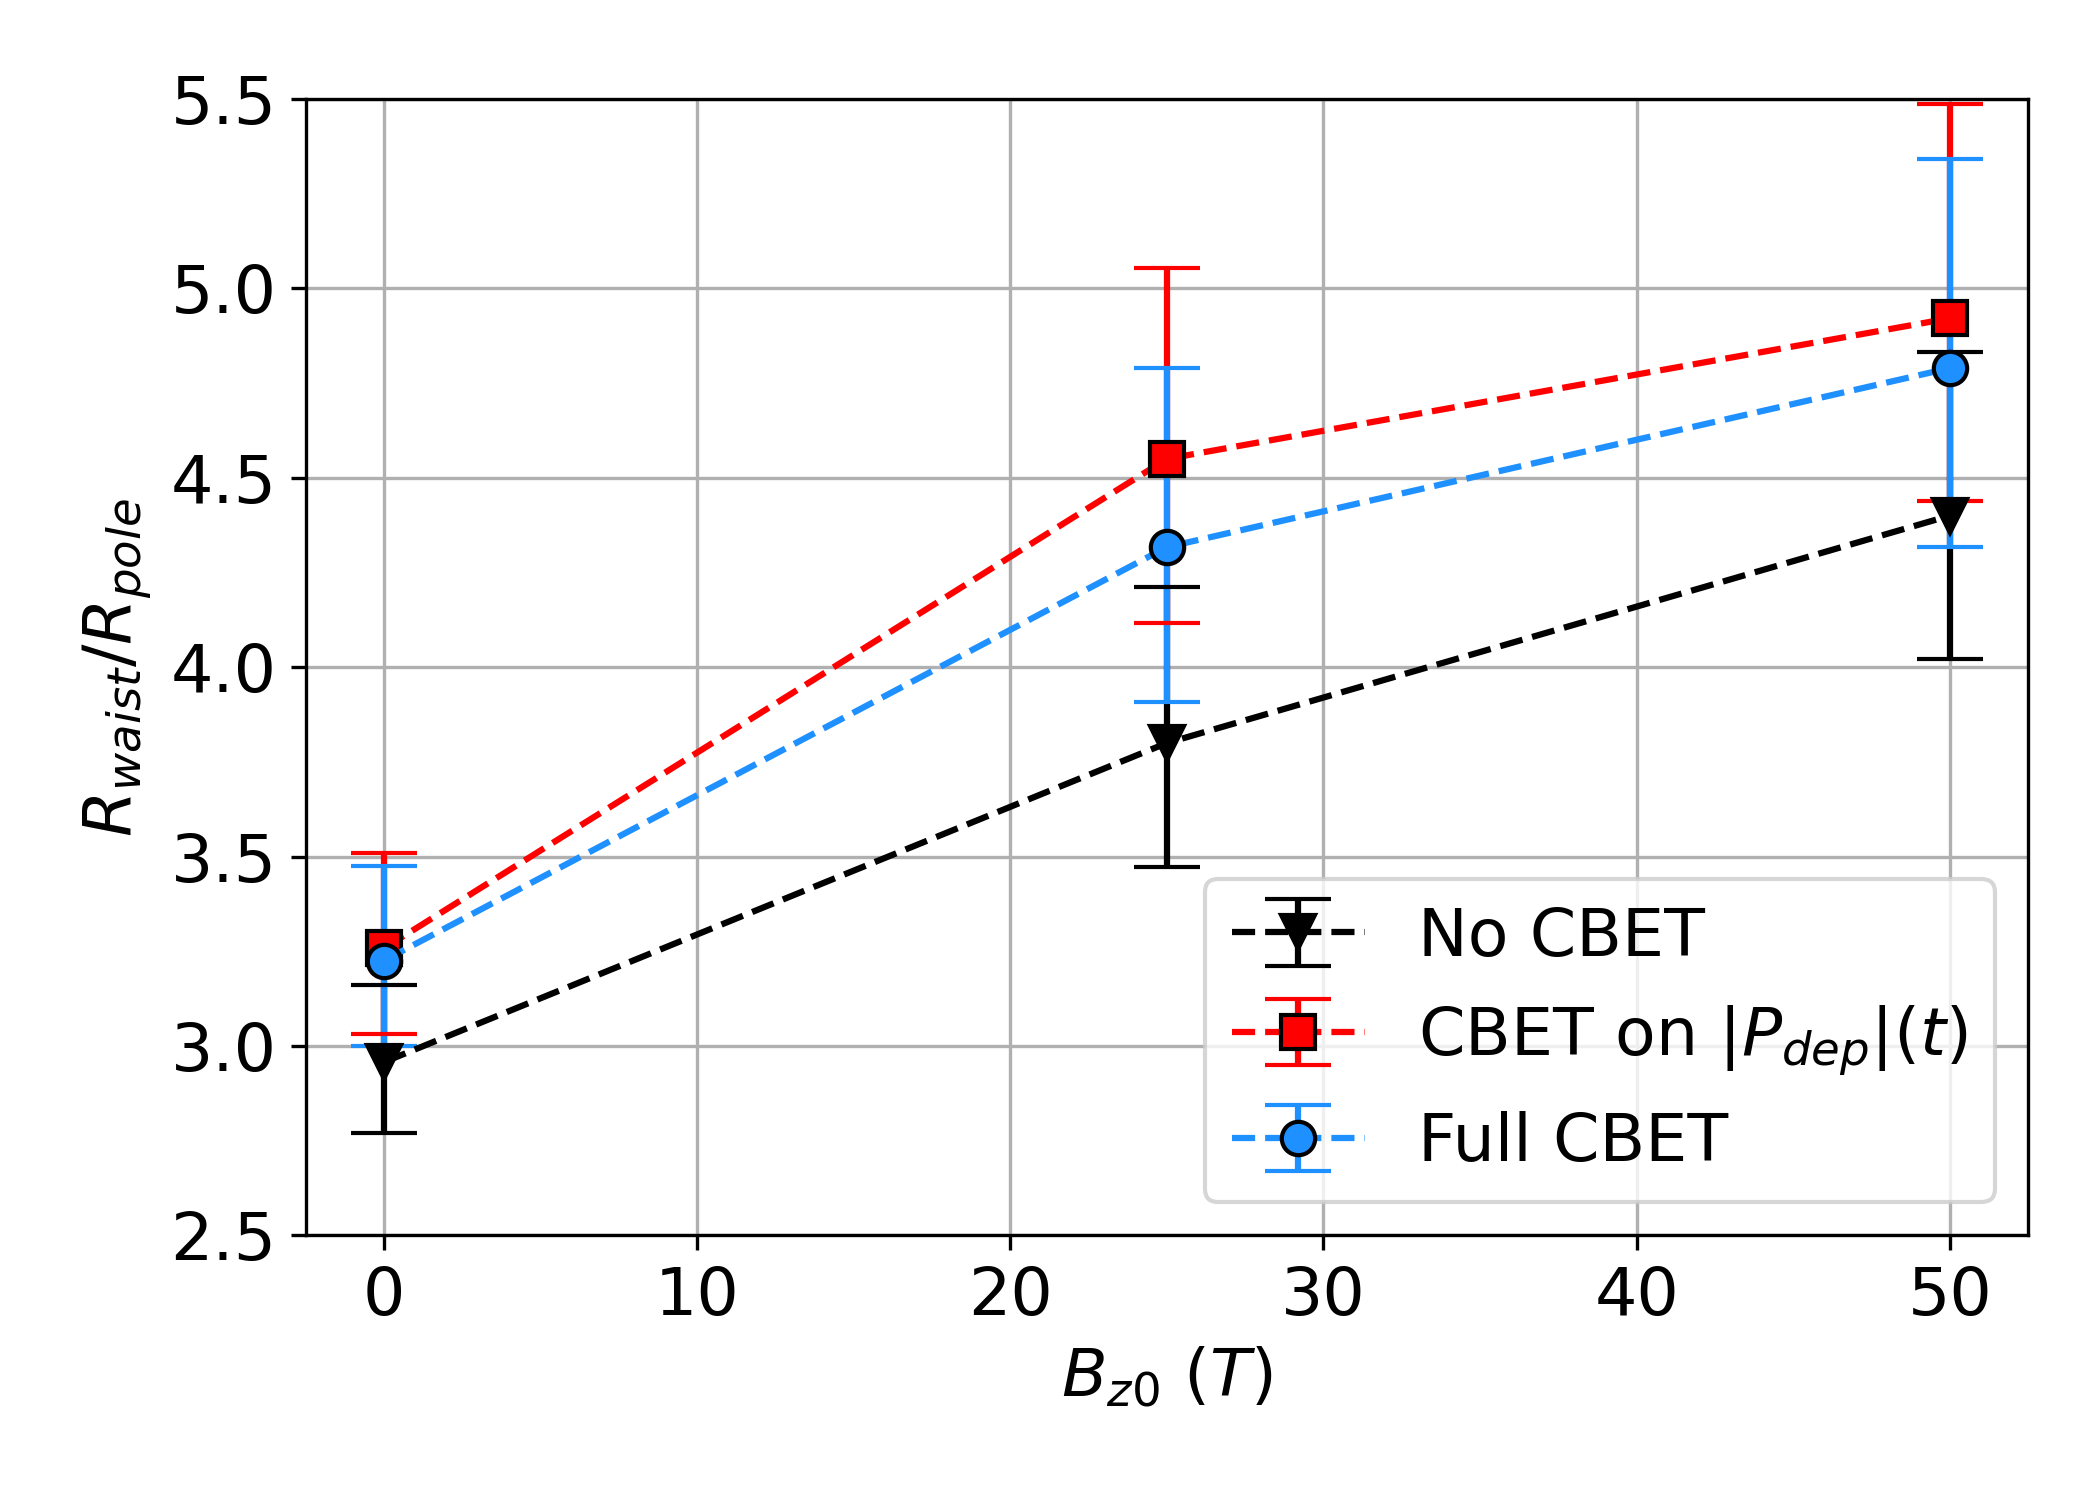
\includegraphics[width=0.7\linewidth]{Results2/Images/R2R0_errors.png}
    \centering
    \caption{lol.}%
    \label{fig:Res2_R2R0_errors}
\end{figure}



%###############################################################################################################################
%###############################################################################################################################
%###############################################################################################################################
\section{Conclusions}%
\label{sec:Res2_conclusions}



%################################################################################
%################################################################################
\subsection{Summary of Work}%
\label{sec:Res2_summary}



%################################################################################
%################################################################################
\subsection{Future Work}%
\label{sec:Res2_future}

